% --------------------------------------------------------------------
% Beamer Template 
% --------------------------------------------------------------------
% Necessary infos for documentstyle
\documentclass[compress]{beamer}

\usetheme{Stud}
\usepackage{times}
\usepackage[utf8]{inputenc}
\usepackage[T1]{fontenc} % nicht benoetigt, in folien wird eh nicht getrennt
\usepackage{ngerman}
\usepackage{graphicx}
%\usepackage{color}% color wird bereits von beamer geladen
\usepackage{verbatim}
\usepackage{psfrag}
\usepackage{math}
\usepackage{calc}
\usepackage{tabularx}
\usepackage{enumerate}
\usepackage{algorithm,algorithmic}


% --------------------------- Helpers ----------------------------
% to use these texts in two languages
% changes the parameter within {#}
% 1 = German
% 2 = English
\def\twolang#1#2{#2} 
\let\2=\twolang

% --------------------------------------------------------------------


\bibliographystyle{alphadin}
\graphicspath{{images/}}


% --------------------------------------------------------------------
\title{Reactive Construction Of Planar, Euklidean t-Spanners With Constant Node Degree}
\subtitle{Antrittsvortrag zur Bachelorarbeit}
\author[T. Budweg]{Tim Budweg}
\institute{
  \texttt{tbudweg@uni-koblenz.de} \\
  \vspace{0.2cm}
  \2{AG Rechnernetze\\
  Universität Koblenz-Landau}{Institute for Computer Science\\
  University of Koblenz-Landau}
}
\date{February 10th, 2016}
% --------------------------------------------------------------------



% document
\begin{document}

\frame{\titlepage}

%\logo{...} erst hier, damit es nicht mit auf die Titelseite kommt!
\logo{\pgfuseimage{logo}}

%\part{Overview}
%\section{\2{Überblick}{Overview}}
%\frame{
%  \frametitle{\2{Überblick}{Overview}}
%  \tableofcontents[part=2,hideallsubsections]
%}

% ====================================================================
% ====================================================================

% here comes the real content which is part of scontent.tex
\part{Content}

% ---------------------------------------------------------------------------
% - For showing graphics and text on one slide use:
%   \begin{columns}[T]
%	\begin{column}[T]{.5\linewidth}
%	    \includegraphics[width=\linewidth]{<filename>}
%	\end{column}
%	\begin{column}[T]{.5\linewidth}
%	    <content>
%	\end{column}
%   \end{columns}
% ---------------------------------------------------------------------------

%\begin{frame}
%\frametitle{}
%\begin{itemize}
%
%\end{itemize}
%\end{frame}

\subsection{Introduction}
\begin{frame}
\begin{itemize}
\item Was ich gemacht habe
\item erklärungen reactive, planar, t-spanner, constant node degree
\item motivation warum ich das gemacht habe
\end{itemize}
\end{frame}

\begin{frame}
\frametitle{Goal}
Algorithm which satisfies the following graph-properties:
\begin{itemize}
\item planar
\item Euklidean t-spanner
\item constant node degree
\item constructed in a reactive way (beaconless, without any prior neighborhood information)
\end{itemize}
\end{frame}

\begin{frame}
\frametitle{Motivation}
Use case: large, static ad-hoc networks (e.g. caution for tsunamis or fire in large areas)
\begin{itemize}
\item reactive: saves a lot of messages
\item constant node degree: safes some more messages
\item theoretical aspect: more properties may lead to possibly better results
\end{itemize}
\end{frame}

\subsection{Algorithm}
\begin{frame}
\begin{itemize}
\item wie der algorithmus läuft
\item rPDT
\item MYS
\item RMYS
\end{itemize}
\end{frame}

\begin{frame} 
\frametitle{rPDT}
	\begin{itemize}
    \begin{columns}[T]
	\begin{column}[T]{.3\linewidth}
    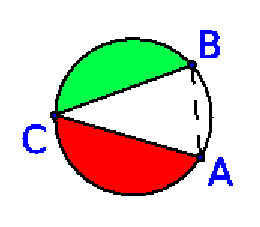
\includegraphics[width=\linewidth]{eigenschaft-beispiel.eps}
	\end{column}
	\begin{column}[T]{.7\linewidth}
	\item Beweis, dass PDT alle modified Yao Step Eigenschaften erfüllt, die $LDel^{(2)}(U) $ erfüllt
	\end{column}
   \end{columns}
	\end{itemize}
\end{frame}

\begin{frame}
\begin{algorithm}[H]
\begin{algorithmic}[0]
\STATE \textbf{Input:} any connected graph $G $; integer $k\geq 14 $
\STATE \textbf{Output:} planar, connected graph $G' $ with constant node degree of at most $k $
\FOR{each node $p \in G $}
\STATE create the PDT-Neighborhood of $p $ using rPDT
\STATE apply rMYS to $p $ using PDT-graph
\STATE let each neighbor of $p $ create its RMYS neighbors and send a protest message if $p $ \indent is not among them causing $p $ to remove this edge
\ENDFOR
\end{algorithmic}
\caption{RMYS}
\end{algorithm}
\end{frame}


\subsection{Results}
\begin{frame}
\begin{itemize}
\item Plots und Erklärung dazu
\item Eigenschaften zeigen
\item Warum formaler Beweis für Spanner nicht geklappt hat.
\end{itemize}
\end{frame}


\end{document}